\documentclass[12pt,a4paper]{report}
\usepackage[utf8]{inputenc}
\usepackage[portuguese]{babel}
\usepackage{titlesec}
\usepackage{graphicx}
\usepackage{indentfirst}
\usepackage{enumerate}
\usepackage{float}
\usepackage{array}
\usepackage{tikz}
\usepackage{multirow}
\usepackage{multicol}
\usepackage{wrapfig}
\usepackage{geometry}
\usepackage[cache=false]{minted}
\usepackage{pdflscape}
\usepackage[titletoc]{appendix}
\usepackage[hidelinks]{hyperref}
\geometry{
 a4paper,
 top=2cm,
 bottom=2cm,
 left=3cm,
 right=3cm
}
\addto\captionsportuguese{
      \renewcommand{\contentsname}
          {Índice}
}
\titleformat{\chapter}{\normalfont\huge}{\thechapter.}{20pt}{\huge}

\begin{document}
\begin{titlepage}
    \center
    {\huge {\bf Universidade do Minho}}\\[0.4cm]
    \vspace{3.0cm}
    \textsc{\huge{Java Factura}}\\[0.5cm]
    \vspace{3.0cm}
    \textsc{\huge{Mestrado Integrado em Engenharia Informática}}\\[0.5cm]
    \vspace{2.0cm}
    \textsc{Programação Orientada a Objectos}\\[0.5cm]
    \textsc{(2º Ano, 2º Semestre, 2017/2018)}\\[0.5cm]
    \vspace{1.5cm}
    \begin{flushleft}
        Grupo 11
        \vspace{1cm}

        A79003 \,\,\,Pedro Mendes Félix da Costa
    \end{flushleft}
        \vspace{1cm}
    \begin{flushright}
        Braga

        Maio 2018
    \end{flushright}

\end{titlepage}

\tableofcontents
\listoffigures

\chapter{Introdução}
    Este trabalho foi realizado no âmbito da unidade curricular programação
    orientada a objectos e teve como objectivo a implementação de um sistema
    similar ao \href{https://faturas.portaldasfinancas.gov.pt}{EFatura},
    aplicando os conceitos leccionados nas aulas.

\chapter{Principais entidades do Sistema}
    \section{Factura}

    \begin{wrapfigure}{r}{5.5cm}
        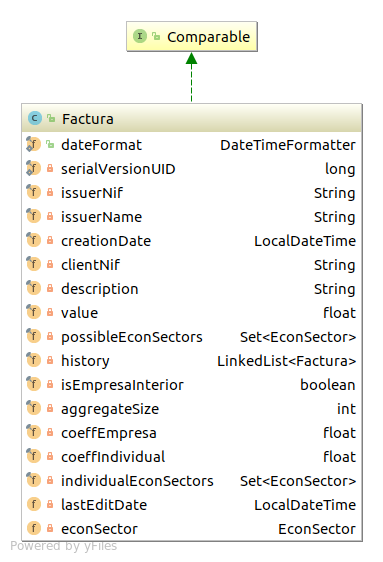
\includegraphics[width=5.5cm]{./images/Factura.png}
        \caption{Diagrama de uma Factura}\label{fig:Factura}
    \end{wrapfigure}

    A classe \mintinline{java}{Factura} representa um documento de despesa no
    sistema. Esta guarda todas as informações pedidas nos requisitos:
    \begin{multicols}{2}
        \begin{itemize}
            \item NIF do emitente
            \item NIF do cliente
            \item Nome do emitente
            \item Data de criação
            \item Valor da despesa
        \end{itemize}
    \end{multicols}
    Além destes, é também guardado um histórico dos estados anteriores da factura
    que é actualizado sempre que o sector de actividade económica desta é
    alterado. A data de edição é também actualizada.

    A alteração do sector económico tem de obedecer a duas restrições para que
    seja executada: 1º uma factura não pode passar a ser Pendente depois de
    emitida e 2º o sector escolhido tem de ser um dos sectores da empresa que a
    emitiu.

    Para além de todos estes dados, uma instância de \mintinline{java}{Factura}
    guarda também alguns dados necessários para calcular a sua dedução. Estes são:
    \begin{itemize}
        \item Se a empresa que a emitiu é uma empresa do interior
        \item O coeficiente fiscal do emitente
        \item O coeficiente fiscal do cliente
        \item O tamanho do agregado familiar do cliente
        \item Os sectores de actividade para os quais o cliente
            pode deduzir.
    \end{itemize}

\pagebreak

    \section{Sectores de Actividade Económica}
    \label{sec:econsector}
    Todos os sectores económicos extendem a classe \mintinline{java}{EconSector}
    que serve apenas para disponibilizar um conjunto de todos esses sectores e um
    método de converter o nome do sector na sua repetiva instância.
    Estas sublcasses por outro lado implementam um padrão \textit{Singleton}, ou
    seja, em qualquer momento existe apenas uma instância de cada um destes
    objectos em memória. A opção pelo padrão \textit{Singleton} foi tomada porque
    estes objectos não têm estado e, como tal, são imutáveis, podendo-se assim
    poupar memória, mas, sobretudo, para ter a garantia que as implementações por
    defeito do \mintinline{java}{equals()} e \mintinline{java}{hashcode()}
    funcionam perfeitamente.
    \begin{figure}[h]
        \begin{minted}{java}
public final class Pendente extends EconSector {

    private static final Pendente instance = new Pendente();
    private Pendente(){}
    public static Pendente getInstance(){
        return instance;
    }
    protected Object readResolve(){
        return getInstance();
    }
}
        \end{minted}
        \caption{Implementação \textit{Singleton} da classe
                \mintinline{java}{Pendente}}
        \label{fig:singleton}
    \end{figure}

    Os sectores económicos estão dividos em duas categorias: dedutíveis
    e não dedutíveis. Esta distinção é feita através de uma interface que
    obriga à implementação do método \mintinline{java}{deduction()} que calcula
    o valor que é deduzido do valor inicial da despesa.
    \begin{figure}[h]
        \begin{minted}{java}
public interface Deductible {
    float deduction(float value, boolean interior, int numDependants,
                    float coeffEmpresa, float coeffIndividual);
}
        \end{minted}
        \caption{Implementação da interface \mintinline{java}{Deductible}}
        \label{fig:deductible}
    \end{figure}

    Os dados necessários a este cálculo são:
    \begin{itemize}
        \item Valor da despesa
        \item Se a factura foi emitida por uma empresa do interior
        \item O número de dependentes do agregado familiar
        \item O coeficiente fiscal do cliente
        \item O coeficiente fiscal da empresa
    \end{itemize}

    \begin{figure}[h]
        \centering
        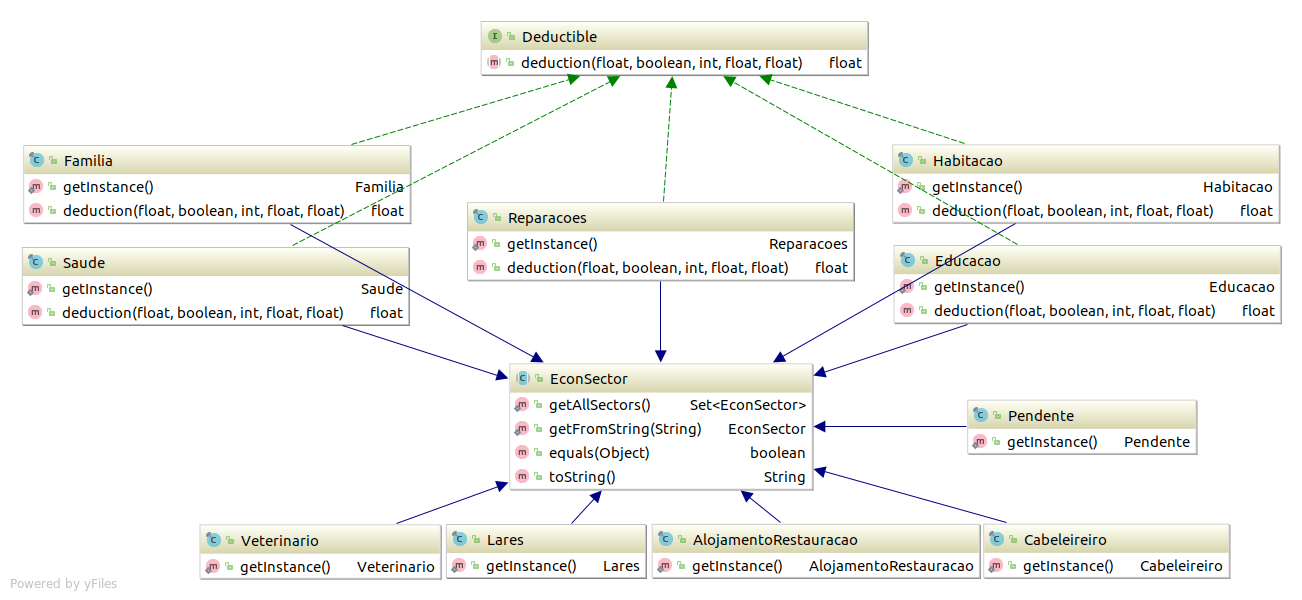
\includegraphics[width=\textwidth]{./images/econSectors.png}
        \caption{Diagrama de classes dos sectores de actividade económica}
        \label{fig:sectors}
    \end{figure}

\pagebreak

    \section{User}
    A interface \mintinline{java}{User} é implementada por duas classes:
    \mintinline{java}{Admin} e \mintinline{java}{Contribuinte}. Esta última, sendo
    uma classe abstracta, é ainda estendida por
    \mintinline{java}{ContribuinteEmpresarial} e
    \mintinline{java}{ContribuinteIndividual}.

    Um \mintinline{java}{User} tem obrigatoriamente de implementar
    \begin{multicols}{3}
    \begin{itemize}
        \item \mintinline{java}{getNif()}
        \item \mintinline{java}{getName()}
        \item \mintinline{java}{getPassword()}
        \item \mintinline{java}{setPassword()}
        \item \mintinline{java}{clone()}.
    \end{itemize}
    \end{multicols}
    Um \mintinline{java}{Admin} implementa apenas a interface, não adicionando mais
    nenhuma funcionalidade. Note-se, no entanto, que o nif e nome do admin são
    sempre iguais a "\mintinline{java}{admin}".

    A classe \mintinline{java}{Contribuinte}, para além de implementar a interface,
    guarda também como variáveis o email, morada, coeficiente fiscal, sectores
    de actividade económica e as facturas. Estes últimos dois atributos são
    vistos de forma diferente dependendo da subclasse que a extende.

    O \mintinline{java}{ContribuinteEmpresarial} acrescenta ao
    \mintinline{java}{Contribuinte} o \mintinline{java}{Concelho} (secção
    \ref{sec:concelho}) onde reside, este podendo ser do interior ou não. Para além
    disto vê as suas facturas como as vendas que realizou e os sectores de
    actividade económica como os possíveis sectores a que essas facturas podem
    pertencer. Este processo de emissão de facturas será explicado em mais detalhe
    na seccção \ref{chp:emissao}.

    O \mintinline{java}{ContribuinteIndividual} acrescenta ao
    \mintinline{java}{Contribuinte} o agregado familiar e define quantos dos seus
    elementos são dependentes. Este vê as suas facturas como as suas despesas e os
    sectores económicos como o conjunto de despesas de onde pode deduzir, tendo a
    capacidade de alterar o sector ecnómico das suas facturas.

    Mais tarde foi também adicionada a noção de \textbf{familia numerosa}, que
    introduz a noção de famílias com mais apoio social, sendo que implementam um
    método que permite reduzir o imposto pago.

    \begin{figure}[H]
        \centering
        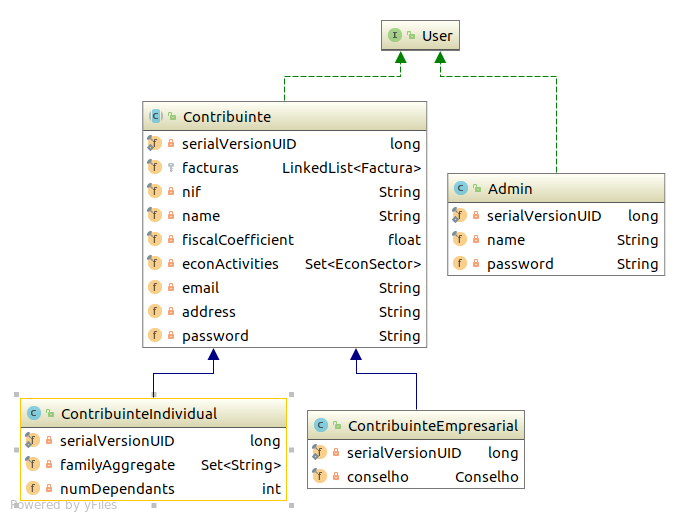
\includegraphics[width=11cm]{./images/UserHierarquy.png}
        \caption{Hierarquia de Classes do \mintinline{java}{User}}
        \label{fig:Hierarquia}
    \end{figure}

\section{Concelhos}
\label{sec:concelho}
    Os concelhos disponíveis são mantidos pela aplicação na forma de um
    \mintinline{java}{enum} que associa a cada um um \textit{boolean} a indicar se
    é um concelho do interior ou não. Desta forma simplifica-se bastante o processo
    de distinção das empresas que são ou não do interior. Para além disto, devido
    ao método como vai ser utilizado, não compromete a extensibilidade do código,
    sendo apenas necessário adicionar novas entradas ao \mintinline{java}{enum}, e
    toda a aplicação mantem o correcto comportamento.

    \begin{figure}[h]
        \begin{minted}{java}
public enum Concelho {
    PORTO(false),
    BEJA(true);
    private boolean interior;
    Concelho(boolean interior){
        this.interior = interior;
    }
    public boolean isInterior(){
        return this.interior;
    }
}
        \end{minted}
        \caption{Excerto do \mintinline{R}{enum Concelho}}
        \label{fig:concelhos}
    \end{figure}

\chapter{Emissão de Facturas e Cálculo de Deduções}
\label{chp:emissao}

\section{Emissão de Facturas}
    Para garantir a consistência do estado interno da aplicação decidiu-se que,
    quando uma factura é emitida, tanto o emissor da factura como o cliente
    deviam guardar a mesma instância do objecto, assim, quando o cliente
    eventualmente alterar o sector económico da factura, esta alteração é
    automaticamente verificada pela empresa. Para que esta arquitetura não
    pusesse em causa o encapsulamento dos dados apenas instâncias de
    \mintinline{java}{ContribuinteIndividual} podem alterar facturas. Esta
    alteração é também muito pequena, tendo muito pouco impacto para a empresa,
    dados os requisitos pedidos.

\section{Cálculo de Deduções}
    A fórmula de cálculo de dedução, como foi referido anterioremente (secção
    \ref{fig:deductible}), fica a cargo dos sectores económicos. Desta forma,
    para que uma despesa seja dedutível, a correspondente factura terá de ser de um
    sector \mintinline{java}{Deductible}
    e de este sector pertencer à lista de sectores para os quais o cliente está
    autorizado a deduzir. Um exemplo de uma destas fórmulas de cálculo pode
    ser vista na \mintinline{java}{Saude}:
    \begin{figure}[h]
        \begin{minted}{java}
public float deduction(float value, boolean interior, int numDependants,
                       float coeffEmpresa, float coeffIndividual){
    float deduction = 0;
    if(numDependants > 1) deduction += 0.3;
    if(interior) deduction += deduction * 1.5;
    deduction += coeffEmpresa + coeffIndividual;
    return value * deduction;
}
        \end{minted}
        \caption{Fórmula de cálculo implementada para o Sector
                    \mintinline{java}{Saude}}
        \label{fig:formulaDeduct}
    \end{figure}

\chapter{Interface Gráfica}

    Quando a aplicação inicia, o primeiro ecrã com que nos deparamos é o de
    \textit{login}. Neste, se introduzirmos as credênciais corretas, leva-nos a um
    dos três ecrãs principais.
\begin{figure}[h]
    \centering
    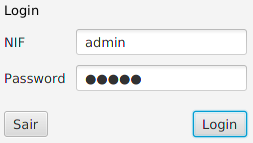
\includegraphics[width=0.4\textwidth]{./images/login.png}
    \caption{Ecrã de \textit{login}}
    \label{fig:login}
\end{figure}

    \section{Admin}
    O ecrã do administrador permite registar novos contribuintes, individuais
    ou empresariais, ver os 10 contribuintes individuais que gastaram mais
    dinheiro até ao momento ou ver os X contribuintes empresariais que mais
    facturas emitiram junto da quantidade monetária facturada.
    Este pode ainda alterar a sua password.
\begin{figure}[h]
    \centering
    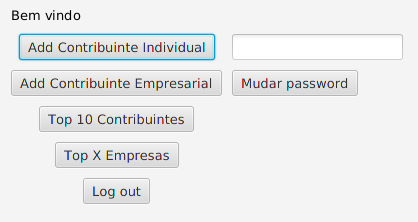
\includegraphics[width=0.5\textwidth]{./images/AdminScreen.png}
    \caption{Ecrã do Admin}
    \label{fig:admin}
\end{figure}

\pagebreak

    \section{Contribuinte Individual}
    O ecrã do contribuinte individual permite consultar o total deduzido por
    si e pelo seu agregado familiar, consultar as suas facturas ordenadas por
    data ou valor e consultar em detalhe cada factura
    (secção \ref{sec:viewFactura}) e alterar o seu sector económico. Pode ainda
    consultar o seu perfil e alterar o seu email, morada e password.

\begin{figure}[h]
    \centering
    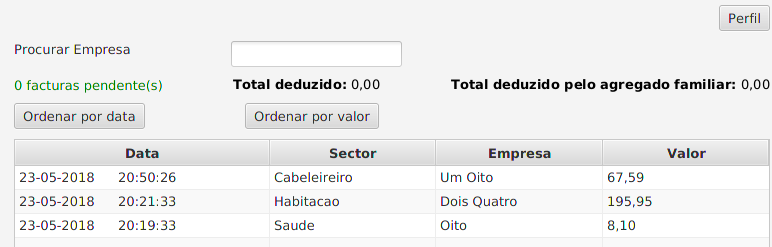
\includegraphics[width=\textwidth]{./images/IndividualScreen.png}
    \caption{Ecrã do individual}
    \label{fig:individual}
\end{figure}

    \section{Contribuinte Empresarial}
    O ecrã do contribuinte empresarial permite consultar o total facturado
    e as facturas emitidas, filtrar ambos por data e ordenar de
    forma análoga ao ecrã do contribuinte individual. Para além disto, permite
    emitir facturas novas e ver a lista dos seus clientes. Ao clicar num dos seus
    clientes pode ver todas as facturas que lhe foram emitidas e, aqui
    também, pode filtrar por data.

\begin{figure}[h]
    \centering
    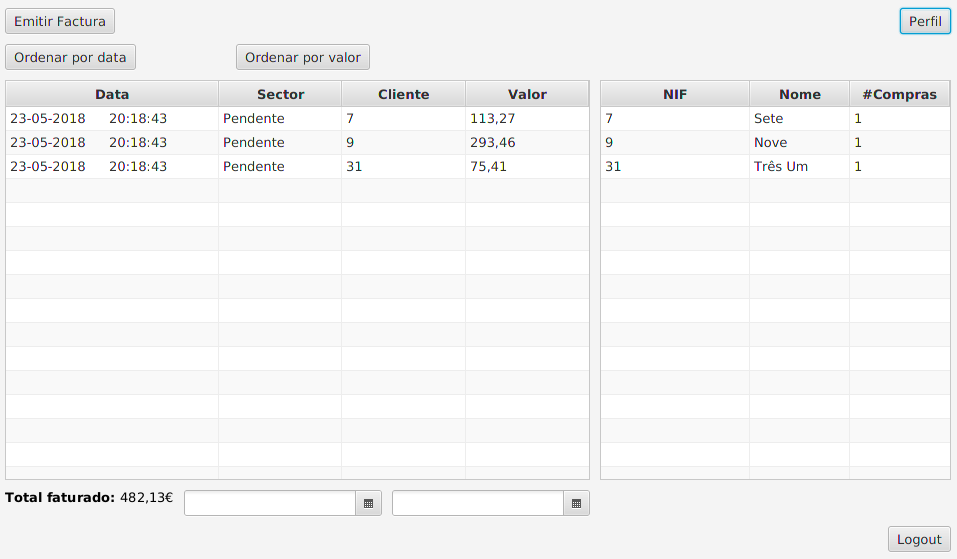
\includegraphics[width=\textwidth]{./images/empresaScreen.png}
    \caption{Ecrã do individual}
    \label{fig:individual}
\end{figure}

    \section{Consultar uma Factura}
    \label{sec:viewFactura}
\begin{wrapfigure}{r}{7cm}
    \centering
    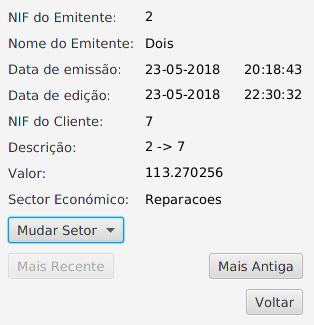
\includegraphics[width=7cm]{./images/facturaView.png}
    \caption{Vista de uma Factura}
    \label{fig:viewFactura}
\end{wrapfigure}
    A consulta de uma factura permite ver todas as alterações que a factura
    sofreu ao longo do tempo e, no caso de o utilizador autenticado ser
    um contribuinte individual, pode também alterar o sector económico desta.

\chapter{Extensibilidade da aplicação}
    A modularidade da arquitetura concebida permite que seja facilmente
    estendida para incluir novos sectores económicos. Basta que seja
    adicionada uma classe que implemente o mesmo padrão \textit{Singleton},
    referido anteriormente (seccao \ref{sec:econsector}), e adicionar esta à lista
    interna da super classe \mintinline{java}{EconSector}. Se esta for dedutível
    basta implementar a interface \mintinline{java}{Deductible}.

\chapter{Conclusões e Trabalho Futuro}
    O trabalho realizado implementa todos os requisitos
    pedidos de forma estruturada, mantendo o encapsulamento dos dados.
\end{document}
